The CASPER people have their own tutorials about a wide-band spectrometer, but we would like to have our own targeting the ROACH2 with the ADC1x5000-8. 

 You can find the CASPER tutorials \href{https://casper.astro.berkeley.edu/wiki/Wideband_Spectrometer}{here} and \href{https://casper-toolflow.readthedocs.io/projects/tutorials/en/latest/tutorials/snap/tut_spec.html}{here}.
 
 
 \section{Some theory}
 As its name says a spectrometer consists in calculate the Fourier transform over certain data and calculate the magnitude of the spectrum.
 
 If you remember the Discrete Fourier Transform (DFT) is defined by \ref{eq:dft}, where N is the size of the DFT and give us the spectral resolution of our spectrometer, k is the channel number and has values ranging from (0,N). 
 A way to view this transformation is defining the twiddle factors $W_{N}^k = e^{\frac{-2\pi i}{N}k}$ which represent the frequency component $\frac{fs}{N}\dot k$ where $fs$ is your sampling frequency. \footnote{In that way the Fourier transform is a change of basis into the $W_{N}^{k}$ base (which is orthogonal)}

So after perform a DFT over a input sequence we have a grid of N frequency points with values $\hat{X}_{k}$. The frequency step would be then $fs/N$.
But there are more caveats, if the input signal is just real you only could use one half of the spectrum calculated. the second half would have repeated information (is the inverted spectrum). So in those cases we just keep N/2 of the calculated channels.
 
 \begin{equation}
     \hat{X_{k}} = \sum_{n=0}^{N-1}x(n)e^{-2\pi i\frac{kn}{N}}
     \label{eq:dft}
 \end{equation}
 
 
 As we mention previously you have a grid of N points in the frequency domain and when the input sequence has a component in one of those specific frequencies you project perfectly only in that specific channel. But what happen when you input sequence has its frequency in the middle of two channels? You could think that it appears in nearest channel, thats partially true.. It gets projected in every channel, but mostly in the close ones, take a look at the figure \ref{fig:leakage} where one of the signals match exactly the frequency and its like a kronecker delta, but the other one that is a little off rise up the other channels. That effect is known as spectral leakage and could be mapped backwards into the orthogonality of the twiddle factors.
 

 \begin{figure}[h]
     \centering
     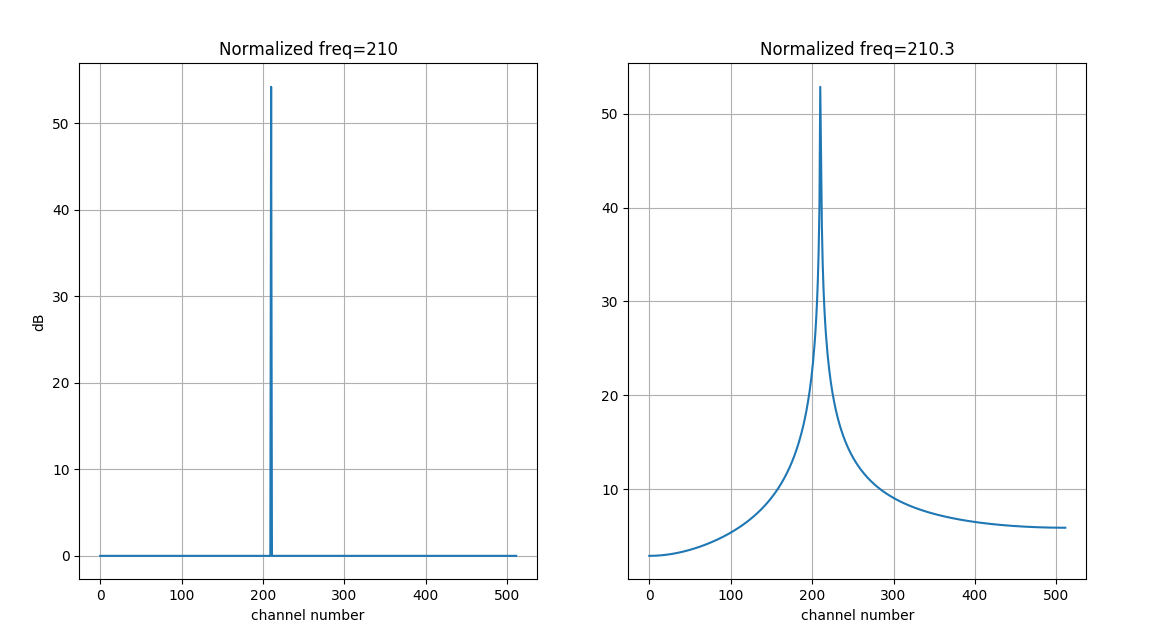
\includegraphics[scale=0.3]{images/leakage.png}
     \caption{Example of spectral leakage}
     \label{fig:leakage}
 \end{figure}

 Anyways, the standard way to explain this effect is that you are actually looking a fixed time interval, so you are computing the DFT over $x(n)w(n)$ where $w(n)$ is a window function. The default window function its just a box shape with ones in the N samples where you are calculate the DFT and zeros elsewhere and the Fourier transform of that is a sync function. So the rectangular window function introduce a main lobe with several side lobes. Those side lobes are the responsible of the spectral leakage, bu the good news is that we could use other window function where the side lobes are lower (remember this effect \emph{cannot be eliminated}, you only can treat it)
 
 
 The CASPER people uses a super nice window scheme using a Polyphase FilterBank which are a bunch of parallel filters structures (check \href{https://arxiv.org/abs/1607.03579}{this} for more info)\footnote{ \href{https://ieeexplore.ieee.org/document/7366712}{This} gives you another usage for PFBs.}
 Also you have to keep in mind that in DSP we always paid the price, normally if we have lower side lobes we have a wider main lobe, if you have a thin main lobe the side lobes are higher and in the PFB we paid with time resolution.
 
 \begin{figure}
     \centering
     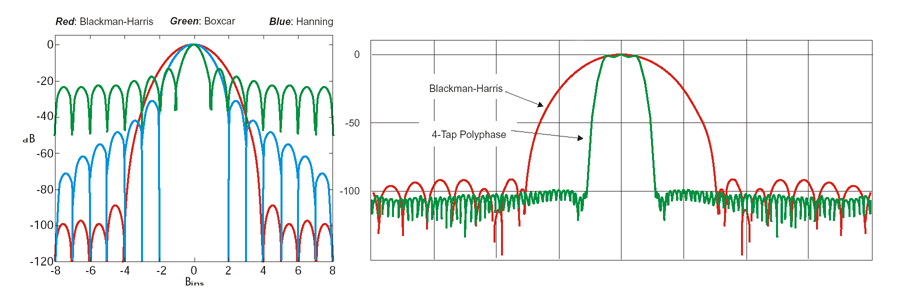
\includegraphics[scale=0.5]{images/pfb.png}
     \caption{Example of different windows spectra taken from \href{https://web.njit.edu/~gary/728/Lecture8.html}{here}.}
     \label{fig:pfb}
 \end{figure}
 

\section{Description of the system structure}

The main advantage of using a FPGA as a spectrometer is that we could collect data meanwhile we are processing it. You have to think this kind of systems as a cascade system where in each clock cycle we have a valid input value and we design everything to be able to handle that requirement.

Also we are not going to deal with multi-clock systems (at least in this upper layer, there are some clock domain crossing here and there, but you don't have to be worried about that, the CASPER people handle it for you). 


The structure is as follows: We have an 8 bit ADC running at 2160MHz, as our FPGA cant handle that clock cycle the ADC give us parallel samples so we are really running the FPGA at a fraction of that sample rate.\footnote{If you have heard about SERDES, here you have one..}

The ADC1x5000 give us 16 samples in each clock cycle, so the FPGA is running at $2160MHz/16 = 135MHz$.
The samples of the ADC are in unsigned format, that means that the data ranges from 0 to 255 where 0 is the most negative value and 255 is the mos positive value, we dont like that representation so our first task will be convert the data to two complement format, which handle positives and negative values.
If you remember $x_{two} = \sim x_{unsign}+1'b1$ makes the trick.


Then with the data in a signed format we feed them into the PFB block and connect the PFB output with the input of the FFT. 
As we mention previously, in each clock cycle we have a new sample available to be process so after a initialization time the PFB and FFTs also deliver a valid output each cycle.


After the FFT we have our spectrum data, but if you look closely the equation \ref{eq:dft} the output is complex and in a spectrometer we only care about the power of the signal. The magnitude of a complex number $z$ is $|z| = \sqrt{\Re e(z)^2+\Im m(z)^2}$, but like performing a square root is expensive in a FPGA and we see the power in dB we just calculate $|z|^2$ (the log doesnt care about the square root and instead of using 20log we are going to use 10log )


We are almost ready. You could use a single spectrum to estimate the parameters of the input signal, but why use just one? It could be useful take average of consecutive FFTs and the FPGA is the best place to do it. 

So we want to compute a FFTs save its magnitude, perform a second FFT, add  each channel with the correspondent channel of the previous FFT and we would like to repeat that process for several frames.
This process involve a memory who saves N samples, wait for the next FFT frame, then reads the saved data and overwrite it adding the incoming data with the saved one, and repeat this process until you reach a given number of FFT frames.
This is known as Bartlett method and is useful to discover signals which are buried in noise\footnote{If the noise is white it grows as $\sqrt{N}$ and a coherent signal would grow as $N$}


Finally we need to take the data out of the FPGA, so we write a two port block memory where one side is connected to the microprocessor in the ROACH system who is going to send the data out by a telnet connection. 


The high level diagram of the system is in the figure \ref{fig:diagram}.

\begin{figure}
    \centering
    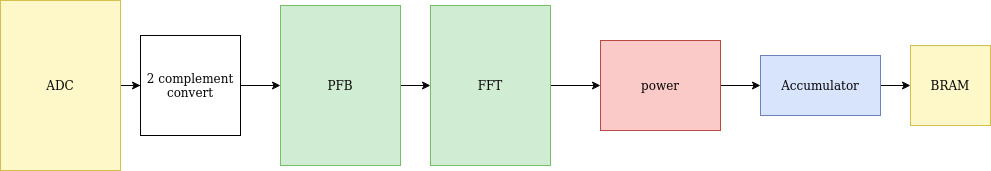
\includegraphics[scale=0.3]{images/diagram.png}
    \caption{High level diagram}
    \label{fig:diagram}
\end{figure}

As a summary:
\begin{itemize}
    \item The adc give us 16 sample each clock cycle and we are running at 1/16 of the sample rate.
    \item We convert the data into signed representation.
    \item We preform a PFB to handle the spectral leakage.
    \item Perform the FFT.
    \item Calculate the magnitude of each FFT channel.
    \item Average multiple FFT frames.
    \item Write the data into a memory block to be read.
\end{itemize}

\section{Simulink blocks}

First a little reminder, the toolflow just works with xilinx blocks and the casper blocks (we also add our own calan\_library that you could use). You could use the other modules of the matlab environment to simulate some stuffs (more of that in another tutorial), but only the xilinx and casper blocks could be synthesized to program the FPGA. 

\subsection{ADC and PFB}

To start, open a new simulink diagram and search for a \textit{system generator} token and then search for
\textit{XSG\_core\_config} and set the clock source to ADC0 and set the clock rate to 135.

Now place a \textit{asiaa\_adc5g} block and set the internal demux as 1:1 and the adc clock rate as 1080.  The input mode is set to One channel, that means that the 16 samples comes from just one sma input. (Setting this to 1:2 will gives you 8 sample from the A input and 8 samples from the C input).

As we mention previously, the sample rate is 2160MHz=2*1080 and our FPGA clock rate is 135=2160/16 (this math is to have everything synchronized to the same ADC clock and to obtain our 16 samples per cycle).

\begin{figure}
    \centering
    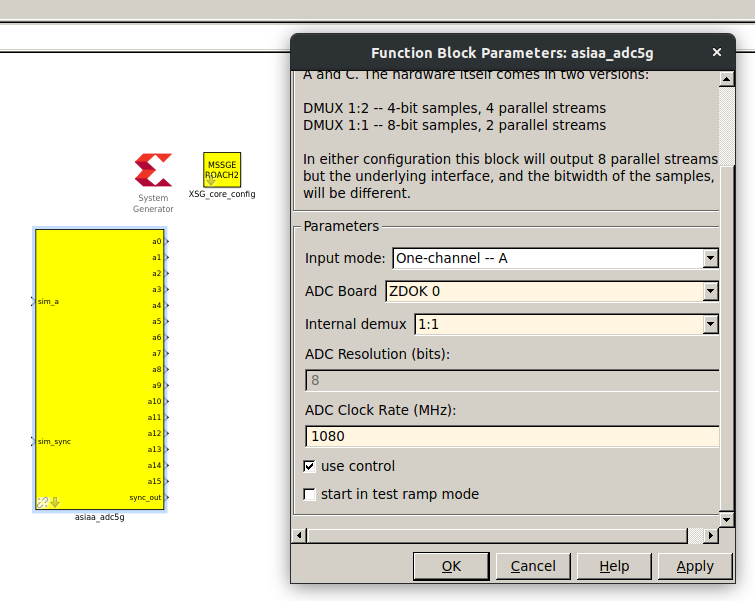
\includegraphics[scale=0.4]{images/asiaa_config.png}
    \caption{Adc 5G configuration}
    \label{fig:asiaa_config}
\end{figure}

Next we need the unsigned to signed conversion, for that we use the \textit{conv} block (its not the same as the \textit{convert} block). Place 16 of those and connect them to the outputs $a_{i}$ of the ADC block. 

To order the diagram you could select all the \textit{conv} blocks, right click and select generate a subsystem.

Now we place a \textit{PFB\_fir\_real} and configure the block as follows.
\begin{itemize}
    \item The size of the PFB is equal to the FFT size, so in our case we will set this to 12 to have 2048 channels (remember, as the inputs are real only we just care about the first half of the FFT).
    \item Set the total number of taps to 4. This is how many parallel filter we will have. You could think that for each FFT frame you are actually feeding the FFT block with $FFT_{size\cdot taps}$
    \item We left the window type to hamming (you could play with it if you want).
    \item Set the parallel inputs to 4 (we have $2^4=16$ simultaneous inputs).
    \item Left the other option as they are.
\end{itemize}

With that, connect the converts with the PFB inputs. See that there is a port named \textit{sync\_in} and other named \textit{sync\_out}, this is a synchronization signal that is going to be used by almost all modules in our signals and arrives to each block \textbf{before} a valid input. The signal is a pulse of a given period, that we will generate after one more step.


\subsection{FFT and sync signal}

Search for \textit{fft\_wideband\_real} block and place itin our design. The modification of the block are:
\begin{itemize}
    \item Number of simultaneous streams: the block support the calculation of several FFTs in the same block (you could share the twiddle factors). As we just have one input we set this as 1.
    \item The size of the FFT should be the same as the PFB, ie 12 which means 2048 channels.
    \item The simultaneous inputs should be 4.
    \item Let the input bitwidth in 18 and set the input binary point to 17.
    \item Its also important that the unscramble output is marked. By default the module has this box checked, this means that the FFT block has its channels sorted (the optimal FFT algorithm doesn't give you the channels in order, os you need to add extra logic to sort it)
\end{itemize}

For each FFT stage you could set a shift to avoid overflow. The standard way to handle it is to shift in every stage. This is controlled by the shift input of the FFT where each bit of the shift input encode if in that stage there is or not a shifting.
We are going to follow the recommendation and put a constant with value 4095 to shift in every stage.
(BTW when configuring the constant value dont forget to mark the sample constant box and set it to unsigned).


Then we proceed to connect the outputs of the PFB with the FFT inputs.


Now we have everything to place the synchronization signal, for that we use the \textit{sync\_gen} block.Check the documentation \href{https://casper-toolflow.readthedocs.io/en/latest/src/blockdocs/Sync_gen.html}{here}. 

Some parameters of this blocks are obvious for example:
\begin{itemize}
    \item FFT len = 4096
    \item PBF FIR taps = 4
    \item FFT sim inputs: 16
    \item We will set the scale to 1. 
\end{itemize}

But there is a weird parameter, the reorder orders. Those are the cost in cycles to sort the FFT channels. To have the values we need to look inside the FFT mask. For that we press the arrow in the bottom left corner of the FFT block. Inside you should see something like the image in the figure \ref{fig:fft_inside}, here we just care about the \textit{fft\_biplex\_real\_4x} and the \textit{fft\_unscrambler}.

We proceed and open the \textit{fft\_unscrambler} to found the image in the figure \ref{fig:fft_scrambler}, where  the important thing is the order number in the \textit{reorder} block. We have to annotate that 8 value.

\begin{figure}
    \centering
    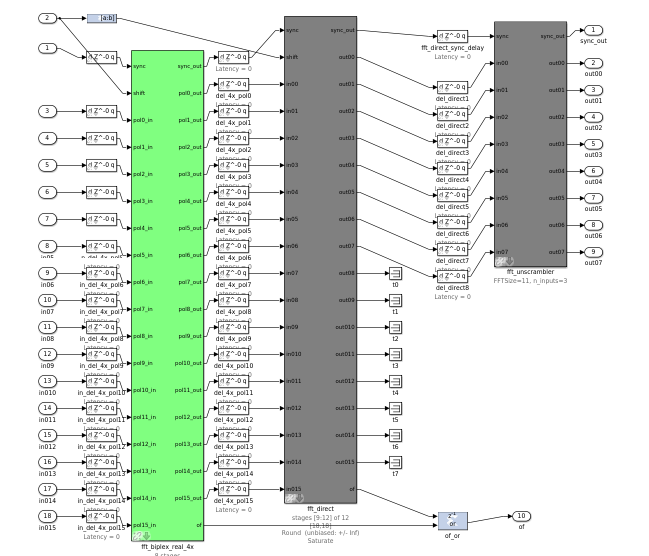
\includegraphics[scale=0.4]{images/fft_inside.png}
    \caption{Inside of the FFT block.}
    \label{fig:fft_inside}
\end{figure}



\begin{figure}
    \centering
    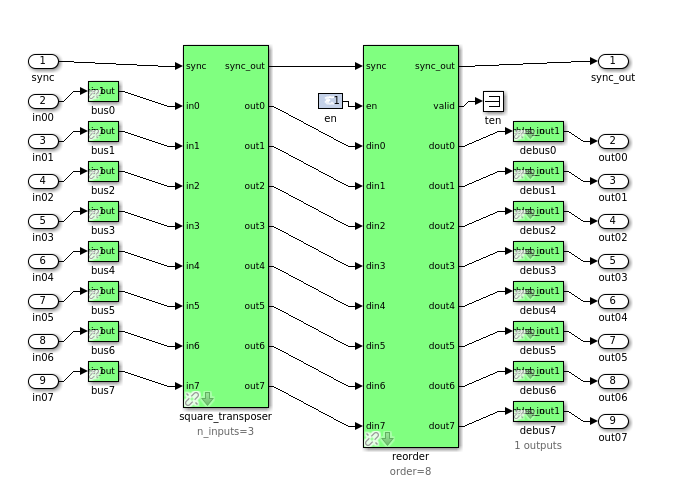
\includegraphics[scale=0.4]{images/fft_scrambler.png}
    \caption{Inside of the FFT scrambler}
    \label{fig:fft_scrambler}
\end{figure}

Now we need to move one step back and return to the FFT mask  and open the \textit{fft\_biplex\_real\_4x} there you will find a block named \textit{bi\_real\_unscr\_4x} which you need to open. The inside of that block is in the figure \ref{fig:bi_unscr}. There, again we annotate the order of the reorder blocks (in this case the even and odd reorders are placed in a parallel way so we just take one).

So as a summary we have the following reorder orders:
\begin{itemize}
    \item \textit{fft\_wideband\_real/fft\_unscrambler/reorder}: 8
    \item \textit{fft\_wideband\_real/fft\_biplex\_real\_4x/bi\_real\_unscr\_4x/reorder\_even} :2 
    \item \textit{fft\_wideband\_real/fft\_biplex\_real\_4x/bi\_real\_unscr\_4x/reorder\_out} :2 
\end{itemize}

With that, the reorder values are [2,2,8]. Typically the reorder\_out and reorder\_even will be 2 but the reorder of the unscrambler change with the FFT size so its always good to review the parameters of your module.
Without a proper sync signal your system will not work!


\begin{figure}
    \centering
    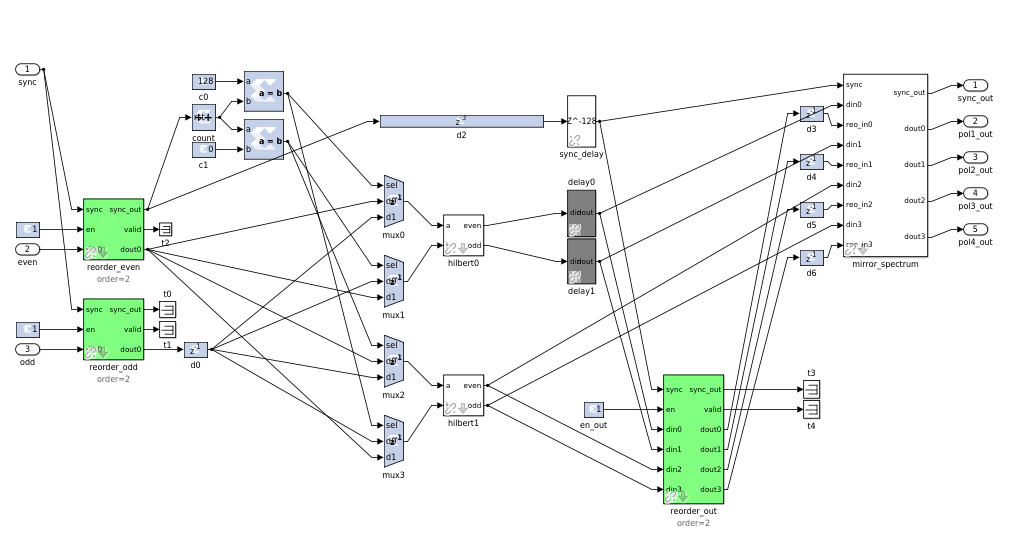
\includegraphics[scale=0.4]{images/bi_unscr.png}
    \caption{Inside of the \textit{bi\_real\_unscr\_4x}.}
    \label{fig:bi_unscr}
\end{figure}

After configure the \textit{sync\_gen} connect the output of that block with the sync input of the PFB. With that we have half of our spectrometer ready and it should looks like the figure \ref{fig:first_half}.

\begin{figure}
    \centering
    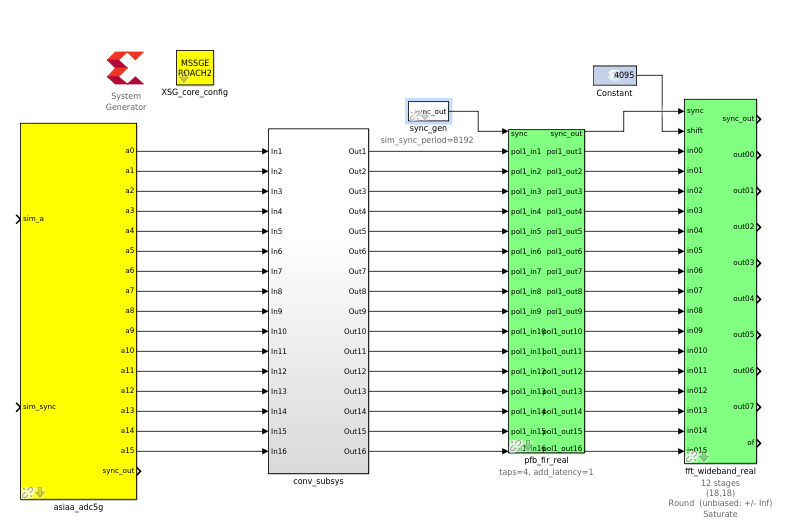
\includegraphics[scale=0.4]{images/first_half.png}
    \caption{ADC+PFB+FFT and sync generator modules}
    \label{fig:first_half}
\end{figure}


Now to follow with the second half we need a timeoff to explain the signal timings to get what we are doing.

\subsection{FFT timing diagrams}
The figure \ref{fig:sync_image} shows the timing diagram where we have a high pulse in the last cycle of the a FFT or in the cycle \textbf{before} a new FFT frame. Also remember that the \textit{FFT\_wideband\_real} gives you only the real part of the spectrum, ie half of the FFT channels, so in the our case the $N$ in the figure \ref{fig:sync_image} is 2048, that also means that every $2048/8=256$ cycles we have a new spectrum available.
Is important to note that the \textit{sync\_gen} period is not necessarily equal to 256, so you could have several FFT frames between two pulses (as we said the FFT is giving you spectra continuously). 


\begin{figure}[t]
    \centering
    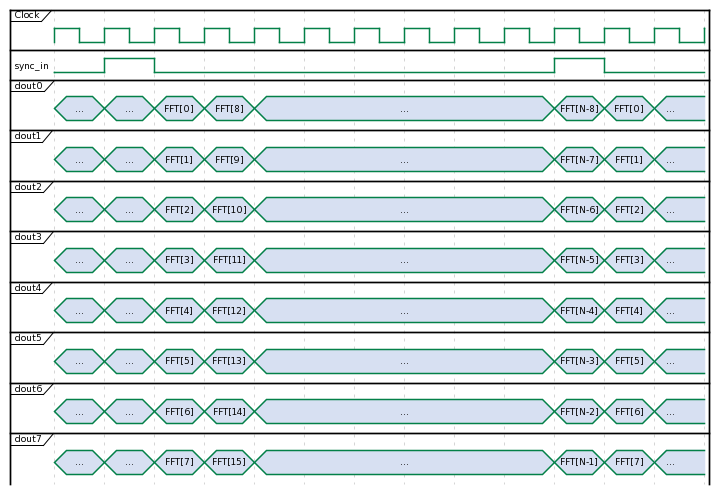
\includegraphics[scale=0.5]{images/sync_timing.png}
    \caption{Sync timing diagram.}
    \label{fig:sync_image}
\end{figure}


Previously we mention that the sync is a reset signal that is passed from module to module, so we will follow that spirit and keep moving the sync signal to synchronize the system.

\clearpage

\subsection{Pipeline and Power}
Now we could continue, first we need to meet one of the most important modules in the toolflow: the \textbf{pipeline}. Open the simulink library and search for it, and place it in every output of the FFT.

The pipeline module is just a bunch of registers, but its importance is because we are dealing with FPGA, so whatever stuff you design at the end should be mapped to the actual components in the FPGA and they have to meet the timing of the clock that you set.
Imagine the following situation, you have a signal that have to travel from the point A to the point B, if you dont put a register in the middle of the path the signal has to cover all the distance in one clock cycle, but if you put in the middle the signal now has one cycle to cover half of the distance. Then the second scheme will help you to achieve the timing closure you need  \footnote{Sometimes placing a register could be a deviation from the path instead of a rest point for example, but the rule of thumbs is that it would help, unless you have a pretty congested area.}




After the pipelines we search for the \textit{power} block, in its mask we have to set the same bit width of the FFT output (18bits). As its name suggest the power block calculate the magnitude of the complex value from the FFT. Connect a power module to the pipilene that comes from the FFT values (dont put it in the sync signal..for obvious reasons).
Now if you look at the power blocks they have a $Z^{-5}$ symbol, that means that to calculate the power of the input it took 5 cycles, so to keep the sync signal synchronized we need to delay it 5 cycles too, so we put a pipeline with a latency of 5.

Now your system should look like the figure \ref{fig:power}.

\begin{figure}
    \centering
    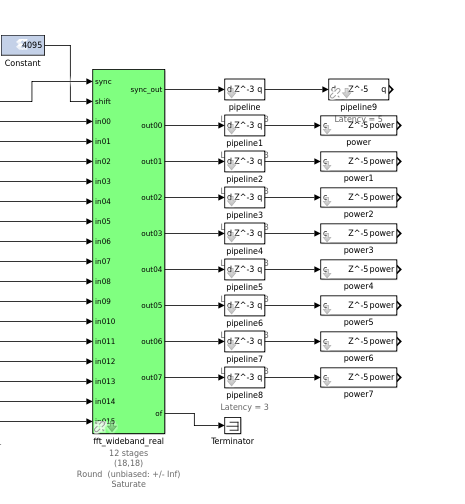
\includegraphics[scale=0.4]{images/power.png}
    \caption{Pipeline and power section}
    \label{fig:power}
\end{figure}



**For an explanation on how to work with the complex data from the FFT take a look at \ref{sec:complex}.

\subsection{Accumulators}
Lets keep moving, we are close to finish. Now following our basic diagram of the figure \ref{fig:diagram} we should average multiple FFTs power outputs.


For that we will need a vector accumulator, search for it as \textit{simple\_bram\_vacc}, but before place it I need to explain how it works because we need another module before it.


The \textit{simple\_bram\_vacc} has two inputs \textit{din}, which you could guess is a data input port, and \textit{new\_acc} port. This blocks does the following: in each cycle that the \textit{new\_acc} port is not asserted it reads from a location in a memory, add the \textit{din} value and finally save the data in the same memory, so if the depth of the memory is correct and everything is synchronized the values that you read and the input values should come from the same channel number achieving our task to accumulate.
Now, when the \textit{new\_acc} port is asserted the block dont add the saved value with the input one, it just save the input value in the memory and the value saved in the memory (ie the accumulated one) goes out on the \textit{dout} port and the \textit{valid} port goes up.


All this is encoded in the timing diagram of the figure \ref{fig:acc_time}, where in that case we accumulate $M$ FFT frames. Note that this timing diagram is for just one dout stream of the 8 from the FFTs.
Is important to note that when the valid signal is not high the data in dout is in an intermediate state.

\begin{figure}
    \centering
    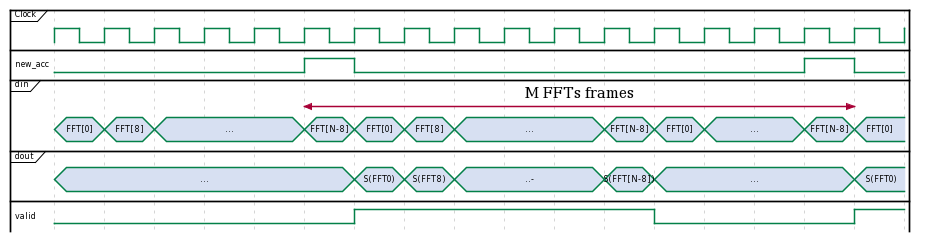
\includegraphics[scale=0.4]{images/acc_time.png}
    \caption{Accumulator timing diagram}
    \label{fig:acc_time}
\end{figure}

So, whats the problem with just connect the sync signal into the new acc?.. 
\vspace{0.1cm}
There will be no accumulation, each frame will pass from the accumulator.

We will need some logic that counts the number of syncs pulses and when it arise to a certain value send a pulse to the new acc. The module that does the job is the \textit{acc\_ctrl}, sarch it and configure it with the the number of channels as 8 (that comes from that we set the FFT length as 12, so the channels will be $2^11$ and as we have 8 parallel streams this will led us with $12-1-3=8$).
The acc\_ctrl has three input ports: the sync that goes connected directly to the delayed FFT sync\_out, the \textit{acc\_len} which is our parameter to set how many FFT frame we will add, the last one is the reset port. In the meanwhile connect the sync ports.


Like we want to have control over the accumulation length and the reset of the system we are going to use the software register to control them. 
Search for \textit{software\_register} and place two of them.


As you should remember from the register tutorials (if you had skipped do it, is super short) the names of the registers and memories are important because we use the names of the simulink blocks to read them from the computer. 
One register will be "acc\_len" and the other one "cnt\_rst" (yes, I am that original).

Now open the dialog box of the "acc\_len" register and set the direction "from processor" and press OK. Also for the "cnt\_rst" set the I/O "from processor" and in the bietfield place put 2 to make the signal boolean.


For visibility we will use a simulink "goto" to not draw to much cables (the reset will be used in other places), the gotos modules gets mapped to the "from " modules, you only have to match the names that you use.\footnote{dont be crazy about using gotos.. simulink got super slow with too many of those bastards.}


With the acc\_ctrl now we could finally place the accumulators. Search a vacc and configure as the image \ref{fig:vacc_parameter}. The vector length is set to 256 because each stream will have $2048/8=256$, the input of the vacc will be an unsigned input of 36 bits with the binary point at 35. So we increase the bit width for the output and maintain the binary point.

\begin{figure}
    \centering
    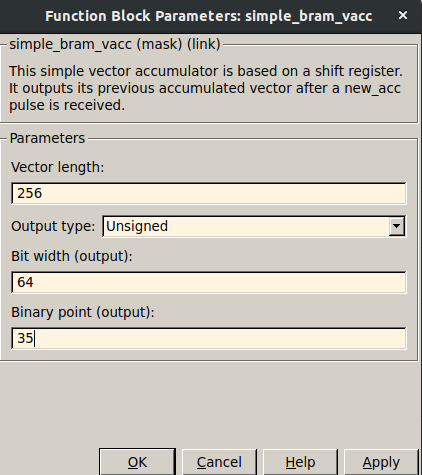
\includegraphics[scale=0.4]{images/vacc_params.png}
    \caption{Vacc parameters}
    \label{fig:vacc_parameters}
\end{figure}


Now you should have something like the figure \ref{fig:vacc_diag} (I add some pipelines though...)

\begin{figure}
    \centering
    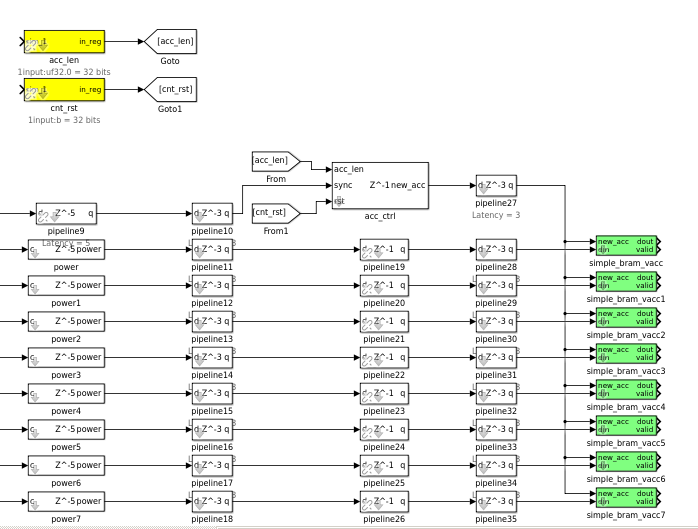
\includegraphics[scale=0.4]{images/vacc.png}
    \caption{System with the vector accumulators and the sync control.}
    \label{fig:vacc_diag}
\end{figure}


\subsection{Brams}


\section{Software side}



\section{Complex data representation digression}
\label{sec:complex}
